\documentclass{article}
\usepackage[utf8]{inputenc}
\parskip = 0.75em
\parindent = 10mm
\def\baselinestretch{1}
\usepackage {float}
\usepackage{listings}
\usepackage{subcaption}
\usepackage[usenames]{color}
\usepackage[numbers,sort&compress]{natbib}
\usepackage{multirow, array}
\usepackage[spanish]{babel}
	\deactivatetilden
	\spanishdecimal{.}
	\addto\captionsspanish{\def\tablename{Tabla}}
	\addto\captionsspanish{\def\listtablename{\'Indice de tablas}}

\usepackage{amsmath,amsfonts,amssymb}
	\allowdisplaybreaks[4]
\usepackage{graphicx}
	\graphicspath{{Figuras/}}
\usepackage[clearempty,pagestyles]{titlesec}
\usepackage{anysize}

\def\baselinestretch{1.5}
\papersize{27.9cm}{21.5cm} 
\marginsize{2cm}{2cm}{1cm}{1cm}

\begin{document}


	\begin{center}
	\huge{\textbf{Tarea 3 Simulación de Teoría de Colas}}
	\line(1,0) {300}\\
	
	\textsc{ \Large Susana Ruiz Nuñez} 
	\textsc{ \Large 2032426}
	\end{center}


\section{Planteamiento de la Teoría de colas} 
Se requiere estudiar el efecto del orden de ejecución de trabajos y el número de núcleos utilizados en la teoría de colas \cite{satu}. La teoría de colas estudia el comportamiento de líneas de espera. Los trabajos que están esperando ejecución en un cluster esencialmente forman una línea de espera. Como medidas de interés principal que ayudan a caracterizar el comportamiento de una línea de espera incluyen el tiempo total de ejecución. 


\section{Metodología}
Se utiliza, en este caso, la examinación de sí o no un número entero dado es un número primo, queriendo decir que no sea divisible entre ningún entero mayor a uno o menor a si mismo. Se comienza con un listado de números primos descargados de la web \cite{mill} y el análisis de si son o no primos con un algoritmo sencillo \cite{satu}. Ya obtenidos la lista de números primos y el análisis para saber si lo son o no, es necesario crear una serie de trabajos fáciles o sea, números que no sean primos que el programa pueda resolver rápidamente.  

Se creó un for para generar una lista de valores que estuvieran entre dos primos grandes; si se tienen dos primos consecutivos, los valores que se encuentran entre ellos no lo son. Estos valores se concatenan junto a los números primos en una lista total que será con la que se seguirá trabajando a continuación.  

\begin{lstlisting}[language=Python]
	facil = []
	for cand in range(minimo+1, maximo-1):
		facil.append(cand)
	total = primos + facil
\end{lstlisting}

Posteriormente era necesario buscar un mecanismo para poder variar el número de núcleos asignados al cluster. El equipo donde se está trabajando el proyecto cuenta con AMD Ryzen 3 3200U with Radeon Vega Mobile Gfx   (4 CPUs), ~2.6GHz, dos núcleos físicos y dos virtuales. Para la variación de los núcleos se utilizaron los paquetes psutil y multiprocessing.

\section{Pruebas Estadísticas}
Se realizaron pruebas estadísticas \cite{jason} para ver la relación existente entre los valores primos obtenidos de la web y los valores no primos generados.

\subsection{Coeficiente de correlación de Pearson}
Se utiliza para comprobar que las dos muestras de valores que estamos tratando estén relacionadas. Prueba la relación lineal entre dos conjuntos de valores.

Supuestos
\begin{itemize}
	\item Las observaciones en cada muestra son independientes y están distribuidas de manera idéntica (iid).
	\item Las observaciones de cada muestra se distribuyen normalmente.
	\item Las observaciones en cada muestra tienen la misma varianza.
\end{itemize}

Interpretación
\begin{itemize}
	\item H0: las dos muestras son independientes.
	\item H1: existe una dependencia entre las muestras.
\end{itemize}

Resultados: Como el coeficiente de pearson $_p > 0.05_$ entonces se plantea que son independientes.

\begin{lstlisting}[language=Python]
	stat=0.420, p=0.580
	Probably independent
\end{lstlisting}

\subsection{Prueba t de Student}
Comprueba si las medias de las dos muestras independientes son significativamente diferentes.


Interpretación
\begin{itemize}
	\item H0: las medias de las muestras son iguales.
	\item H1: las medias de las muestras son desiguales.
\end{itemize}

Resultados: Como el coeficiente de pearson $_p > 0.05_$ entonces se plantea que tienen la misma distribución.

\begin{lstlisting}[language=Python]
	stat=1.452, p=0.242
	Probably the same distribution
\end{lstlisting}

\section{Resultados}
Como se muestra en la (Figura 1) hay una diferencia considerable en los tiempos de ejecución, se muestra mucho más al aumentar los núcleos que en los diferentes tratamientos de los datos, se trataron de manera Normal, es decir, en el orden que aparecen en la lista, luego de manera Inversa y finalmente aleatoriamente. En el caso del uso de los núcleos se muestra como se acercan a 0 mientras más núcleos se utilizan. Se da una muestra de los datos obtenidos con el uso de Python3.7, para un núcleo y para cuando se utilizaron los 4 núcleos.

\begin{lstlisting}[language=Python]
DescribeResult(nobs=10, minmax=(0.49785828590393066, mean=0.8369509935379028)
DescribeResult(nobs=10, minmax=(0.500037670135498, mean=0.6482812881469726)
DescribeResult(nobs=10, minmax=(0.5040359497070312, mean=0.6433071374893189) 
\end{lstlisting}
.
.
.
\begin{lstlisting}[language=Python]
DescribeResult(nobs=10, minmax=(0.32102465629577637, mean=0.5686076641082763)
DescribeResult(nobs=10, minmax=(0.32302260398864746, mean=0.3506206512451172)
DescribeResult(nobs=10, minmax=(0.3180241584777832, mean=0.3628715753555298)
\end{lstlisting}
\begin{figure}
	\centering
	\begin{subfigure}[b]{0.45\linewidth}
		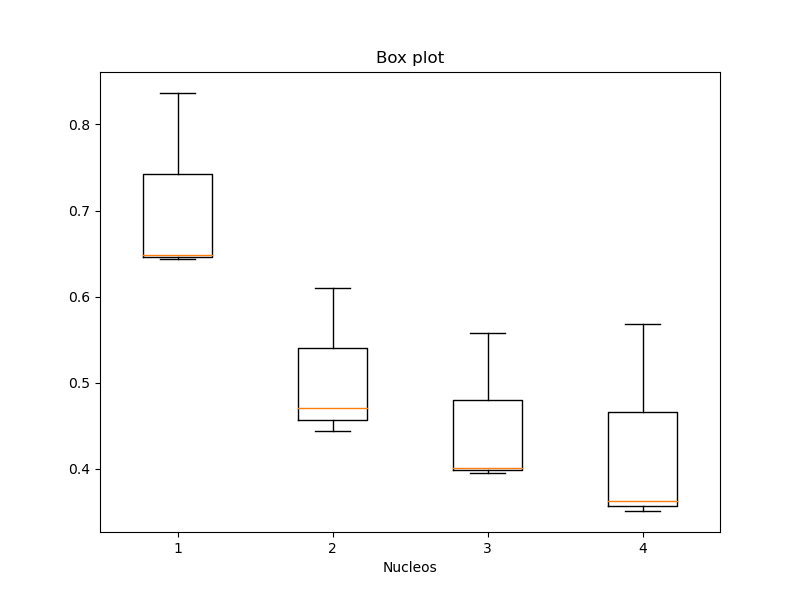
\includegraphics[width=\linewidth]{Figure_1.png}
		\caption{Utilización de núcleos.}
		\label{32pasos}
	\end{subfigure}
		\begin{subfigure}[b]{0.45\linewidth}
		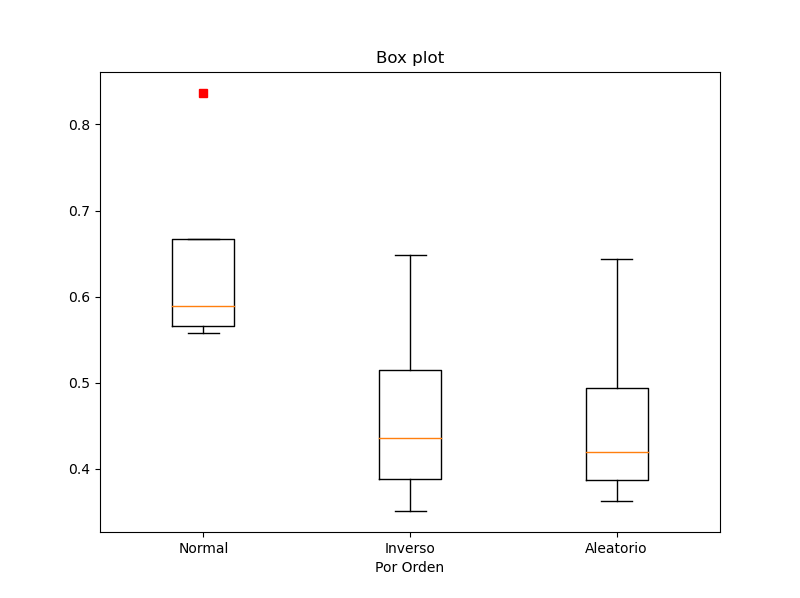
\includegraphics[width=\linewidth]{Figure_2.png}
		\caption{Orden de los datos.}
		\label{1024pasos}
	\end{subfigure}
	\caption{Resultados por utilización de núcleos y orden de los datos.}  		
\end{figure}


En la (Figura 2) se muestra el comportamiento  por el Ordenamiento a que fueron tratados los datos. Se nota a simple vista que cuando el Orden tenía los números primos delante era más complejo el análisis de los datos. Lo que cambia al invertir el orden y tratar los valores fáciles primero y de manera aleatoria.

\begin{figure}[H]
	\centering
	
	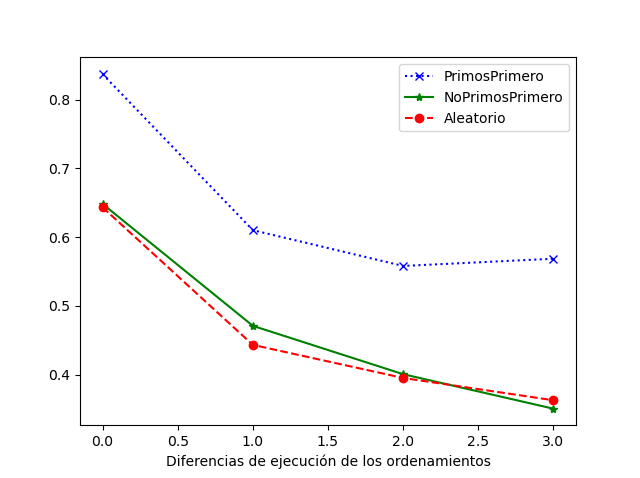
\includegraphics[scale=0.6]{Figure_3.png}
	\caption{Ejecución por Orden}
	\label{fig:f2}
\end{figure}

\section{Conclusiones}
Se puede concluir con los experimentos realizados que al aumentar el número de núcleos asignados al cluster, se realiza un mejor trabajo de procesamiento observándose gran diferencia en los tiempos de procesamiento. Lo mismo ocurre en el ordenamiento de los datos, si se juega al tetris con las fichas más difíciles al inicio se hará más complejo el trabajo a la pc.

\bibliography{Tarea3}
\bibliographystyle{plainnat}
\end{document} 
